\chapter{Discussão sobre esquemas adequados de redundância de dados}

Pode-se encontrar na literatura um número significativo de projetos que propõem sistemas de armazenamento distribuído, sistemas de arquivos distribuídos, ou sistemas de backup. Apesar da disso, nenhum esquema de redundância de dados tem sido amplamente aceito para esses sistemas e nenhuma regra fácil foi criada para se encontrar um esquema adequado de redundância de dados.

Para implementar redundância de dados em sistemas, são utilizadas
várias técnicas: codificação por apagamento, replicação, espelhamento,
\emph{Cyclic redundancy check} (CRC), \emph{bits} de paridade,
\emph{checksum} e assinatura digital. Esquemas de
redundância podem implementar um conjunto destas
técnicas~\cite{Fan:2009}.

Os autores em \cite{Duminoco:2009} estudaram redundância de dados em sistemas \emph{peer-to-peer} para \emph{backup} e propuseram um esquema hídrido para implementar redundância (replicação e codificação) de dados. Em \cite{Storer:2008}, foi proposto um sistema de armazenamento de dados baseado em discos que usa dois níveis de codificação. Nesses textos, encontramos uma comparação entre alguns sistemas de armazenamento, avaliando-se algumas de suas características. Podemos observar que os tipos de esquema de redundância de dados são replicação, codificação por apagamento e híbrido, sendo a replicação, a estratégia mais utilizada nos sistemas comparados por \cite{Duminoco:2009} e a codificação por apagamento, para os sistemas comparados por \cite{Storer:2008}.

Redundância de dados é necessária para prevenir perda de dados, mas não é suficiente. A avaliação de esquemas de redundância é muitas vezes baseada na suposição de que as réplicas falham de forma independente. Na prática, as falhas não são tão independentes, segundo \cite{Weatherspoon:2002:02,Baker:2006}. Esse trabalho não tratará a independência das réplicas.

Cada esquema de redundância estabelece (i) como criar os dados redundantes e (ii) como reconstruir os dados quando houver falha. Essas duas operações geram custos que diferem de um esquema para outro. Esse trabalho comentará os mais amplamente usados esquemas de redundância: replicação e codificação por apagamento, que chamaremos de codificação.

\section{Esquemas de redundância de dados para sistema de armazenamento}

Esquemas de redundância de dados são utilizados em sistemas de armazenamento (exemplo: sistemas RAID) para prover disponibilidade, tolerância a falhas e durabilidade de dados e em sistemas de comunicação (exemplo, sistemas \emph{peer-to-peer}) para prover uma entrega confiável e segura de dados.

A Figura~\ref{fig4:srp} apresenta um sistema de armazenamento com um arquivo de dados particionado em 8 blocos. O fator de replicação é 4. Os clientes precisam que, para cada um dos 8 distintos blocos, uma das quatro cópias esteja disponível. A Figura~\ref{fig5:crs} apresenta o mesmo sistema que a Figura~\ref{fig4:srp}, mas utilizando códigos RS. O arquivo está particionado em 8 blocos e 32 blocos codificados foram gerados. Os clientes podem utilizar quaisquer 8 blocos para obter o arquivo inicial. A Figura~\ref{fig5:crs} também se aplica a códigos Tornado.

   \begin{figure}[h]
     \centering
     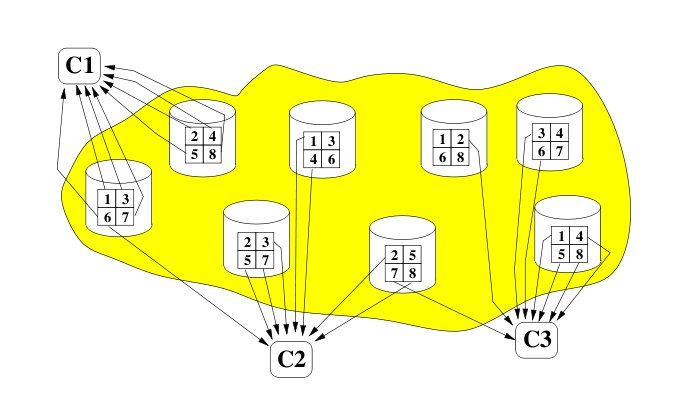
\includegraphics[scale=.6]{figuras/replicacao-pura.jpg}
     \caption{Sistema com replicação pura \cite{Plank:2004}}
     \label{fig4:srp}
   \end{figure}

   \begin{figure}[h]
     \centering
     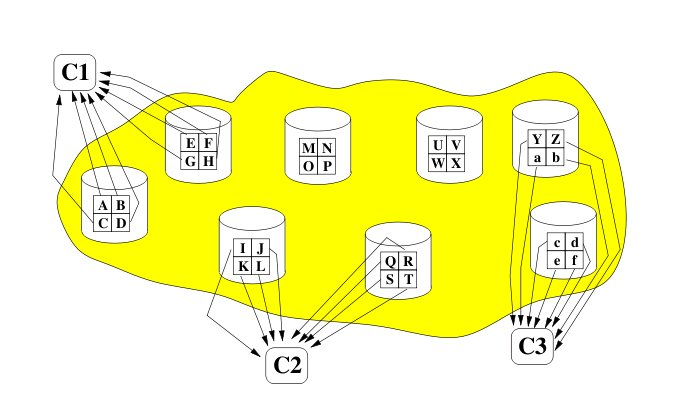
\includegraphics[scale=.6]{figuras/codigos-RS.jpg}
     \caption{Sistema com códigos RS \cite{Plank:2004}}
     \label{fig5:crs}
   \end{figure}

\subsection{Replicação}

Replicação é o esquema de redundância mais simples. A maioria dos sistemas, que utiliza redundância de dados, é baseada em replicação, mas esse esquema consume mais espaço que a codificação por apagamento, pois uma cópia completa de cada arquivo é armazenada em cada um dos servidores de dados.

A principal desvantagem da replicação é que ela requer uma grande sobrecarga de armazenamento para pouco ganho em disponibilidade e tolerância a falhas. Garantir que os dados permaneçam disponíveis quando todos os $n$ dispositivos falham exige que, pelo menos, $n + 1$ cópias existam \cite{Woitaszek:2007}. Por exemplo, no artigo sobre o sistema Glacier \cite{Haeberlen:2005}, os autores argumentam que o armazenamento aumenta de 11 vezes a quantidade de dados armazenados utilizando apenas replicação para conseguir 0.999999 (\emph{six nines}) de confiabilidade num cenário com 60\% de indisponibilidade dos nós.

Os autores em \cite{Dabek:2004} afirmam que dados replicados permitem leituras de baixa latência, porque há muitas opções para a seleção de servidores, enquanto que dados codificados reduzem o consumo de largura de banda para escritas, em detrimento do aumento da latência de leituras.

A replicação é usada no Google File System \cite{Ghemawat:2003} (GFS), no Hadoop Distributed File System \cite{Hadoop:2010} (HDFS) e no Kosmos distributed file system \cite{TKDFS:2011} (KFS), sistemas de arquivos distribuídos que apresentam características semelhantes. Um \emph{cluster} do GFS ou do HDFS ou do KFS é formado por um único servidor, master (GFS) ou namenode (HDFS) ou Meta server (KFS), que mantém os metadados e muitos servidores de dados, os chunkservers (GFS e KFS) ou os datanodes (HDFS) e é acessado por vários clientes. Os arquivos de dados são armazenados nos chunkservers (GFS e KFS) ou datanodes (HDFS) e são particionados em blocos de igual tamanho. GFS, HDFS e KFS foram projetados para aplicações que processam grande volume de dados. 

Seus projetos consideram \emph{clusters} de (\emph{commodity hardware}), uma versão do \emph{kernel} linux como sistema operacional para as máquinas e uma arquitetura de rede com dois níveis: vários \emph{racks} interligados por um comutador e cada \emph{rack} é formado por várias máquinas e seus discos, estes também interligados por um comutador. A estratégia de inserção de dados cria réplicas em \emph{racks} distintos do \emph{rack} onde está a 1$^a$ réplica, assim, falhas que comprometam um \emph{rack} não provocam a indisponibilidade de dados. Os arquivos de dados são alterados por concatenações ao invés de sobrescrever dados existentes. Após a criação, os arquivos de dados são usados apenas para leitura e esta leitura ocorre sequencialmente. O KFS permite escrever em posições randômicas nos arquivos. As APIs do cliente fornecidas pelo GFS, pelo HDFS e pelo KFS suportam operações de criação, leitura, escrita, remoção de arquivos, mas não implementam a interface POSIX.

O GFS está disponível para linux sob uma licença de software proprietário. O HDFS \footnote{http://hadoop.apache.org/}  e o KFS \footnote{http://code.google.com/p/kosmosfs/} estão disponíveis para linux sob uma licença Apache. 

O Farsite, que utiliza apenas replicação, é um sistema de arquivos distribuídos, particionados em namespaces, explorando os desktops presentes dentro da Microsoft, sem servidor mestre, disponível para Windows sob uma licença de software proprietário. A escolha da replicação foi, pelos autores, considerada uma opção mais simples para disponibilidade, já que a codificação poderia significar latência adicional nas leituras dos arquivos. Ainda segundo os autores, estudos com experimentos já mostraram que a codificação pode apresentar um bom desempenho e seria possível, então, alterar no futuro o esquema de redundância do Farsite.

Big Table (construído sob o GFS) e Dynamo (construído para Amazon.com) são dois sistemas de armazenamento que gravam e recuperaram dados através de uma chave e executam em um \emph{pool} compartilhado de máquinas, utilizam apenas replicação. 

Ceph \cite{Weil:2006} é um sistema de arquivos \emph{open source} que possui três principais componentes: um \emph{cluster} de servidores de metadados (que gerencia o namespace, nomes de arquivos e diretórios), um \emph{cluster} de OSDs (dispositivos de armazenamento de objetos) que armazenam dados e metadados e os clientes que utilizam uma interface do sistema de arquivos. O Ceph agrupa dados em PGs (grupos de colocação) e usa uma função \emph{hash} para distribuir os PGs nos OSDs, cujo algoritmo CRUSH é $O(log n)$ e usa uma árvore-B para indexar os PGs. Existe um módulo em desenvolvimento que permite usar o Ceph como armazenamento para uma instância do Hadoop. O Ceph utiliza apenas replicação, implementa parcialmente a interface POSIX e está disponível para linux sob LGPL \footnote{http://ceph.newdream.net/}.

Lustre \footnote{git://git.lustre.org/prime/lustre.git} tem na sua arquitetura os metadata server (disponibiliza os metadados para clientes), o metadata target (um por sistema de arquivos, armazena os metadados), object storage servers (armazena os dados), object storage target (armazena os objetos que contém os arquivos de dados) e clientes.

Moosefs \footnote{http://www.moosefs.org/} também foi projetado com uma arquitetura que se assemelha a do GFS, HDFS e KFS: master server (que armazena os metadados), chunk servers (que armazenam os dados), metalogger server (podem substituir algumas funções do master server, se ele falhar) e clientes (que solicitam dados e se comunicam com o master server e o chunk servers. 

Ambos, Lustre e Moosefs, usam replicação, implementam a interface POSIX e estão disponíveis para linux sob uma licença GPL.

Com exceção do Farsite, os sistemas de armazenamento apresentados consideram \emph{clusters} de (\emph{commodity hardware}) e uma versão do \emph{kernel} linux como sistema operacional para as máquinas.

\subsection{Codificação por Apagamento}

Uma vantagem de codificação por apagamento é um custo menor de armazenamento se comparado a replicação, no caso de grande volume de dados. Outra vantagem com relação a replicação foi comentada em \cite{Weatherspoon:2002:01}: para um mesmo espaço de armazenamento, o tempo médio entre falhas (\emph{mean time to failure}) é maior.

\begin{table}
%\singlespacing
    \centerline{
    \begin{tabular}{|p{2cm}|p{4cm}|p{5cm}|p{2cm}|}\hline
	{\bf sistema} & {\bf codifica��o} &  {\bf arquitetura do sistema} & {\bf licen�a}\\ \hline
	HDFS \cite{Hadoop:2010}& RAID, RS, ... & shared-disk file system for cluster & Apache\\ \hline
	Tahoe-LAFS \cite{Wilcox-O'Hearn:2008} \footnote{http://tahoe-lafs.org/trac/tahoe-lafs} & RAID & peer-to-peer filesystem & GPL2\\ \hline
	Pergamum \cite{Storer:2008}& XOR parity, RS &  disk-based archival storage & *\\ \hline
	Potshards \cite{Storer:2009} & RAID e RS &  disk-based archival storage & *\\ \hline
	RobuStore \cite{Xia:2006} & Luby Transform (LT) & disk-based archival storage & *\\ \hline
	Glacier \cite{Haeberlen:2005}& RS com matrizes Cauchy & peer-to-peer storage system & *\\ \hline
	Total Recall \cite{Bhagwan:2004} & Maymounkov's online codes &  peer-to-peer storage system & *\\ \hline
	FAB \cite{Saito:2004}& RS & distributed disk array & *\\ \hline
	GPFS \cite{Schmuck:2002}& RAID & shared-disk file system for cluster & *\\ \hline
	Oceanstore \cite{Kubiatowicz:2000} \footnote{http://oceanstore.sourceforge.net/}& Tornado e RS & desktops e notebooks conectados a servidores geograficamente distribu�dos & BSD \\ \hline
	xFS \cite{Anderson:1998} \footnote{http://oss.sgi.com/projects/xfs/} & RAID & serverless network file system & GPL\\ \hline
	Swift \cite{Cabrera:1991} & RAID & desktops sob unix conectados a uma intranet & *\\ \hline
    \end{tabular}}
    \caption{Compara��o de codifica��o entre sistemas de armazenamento de grande volume de dados que utilizam \emph{commodity hardware}}
    \label{tab1:comp}
    onde:\\
    * = n�o dispon�vel
\end{table}


HDFS, Total Recall e OceanStore usam codificação para reduzir o tamanho do armazenamento de dados e todos os outros sistemas usam codificação para prover disponibilidade e confiabilidade.

Os sistemas que foram comparados na tabela ~\ref{tab1:comp}, estão disponíveis para uma versão de sistema operacional linux ou unix. Além da codificação, todos eles implementam replicação.

Vamos avaliar algumas das métricas utilizadas em literatura para comparar redundância de dados em sistemas de armazenamento: sobrecarga de armazenamento, disponibilidade dos nós, corrupção de um dado e operações de criação, leitura, atualização consistente e remoção de dados redundantes. Inicialmente vamos definir alguns conceitos adaptados de \cite{Duminoco:2009, Chiola:2005, Rodrigues:2005, Williams:2007} para esses dois esquemas de redundância.

\section{Caracterização da replicação e da codificação}

A confiabilidade de um esquema de redundância é medida pelo número de falhas simultâneas que ele pode tolerar sem comprometer a capacidade de reconstruir os dados originais. Assim esta propriedade pode ser expressada como a {\bf probabilidade de perda de dados, dado que ocorreram $l$ falhas}, $P(l)$.

Para avaliar o armazenamento, vamos definir {\bf fator de redundância} $B$, uma razão entre tamanho dos dados originais mais a redundância $|dado\ +\ red|$ e o tamanho dos dados originais $|dado|$ e também vamos definir grau de reparação.

O {\bf grau de reparação} mede o que deve ser feito após parte da redundância ser perdida. Para isso, é feita uma leitura de dados disponíveis para produzir novos. O custo dessa leitura em um sistema de armazenamento distribuído inclue volume do tráfego da rede, política de reparação, algoritmo de coordenação. Nesse estudo vamos apenas avaliar a contribuição do esquema de redundância: a quantidade de dados a serem lidos para que dados novos sejam criados para reparar o dado corrompido, definido por $d$.

Definimos $p$ como a probabilidade de um nó estar disponível e  $q\ =\ 1\ -\ p$ como a probabilidade de um nó não estar disponível. Nesse estudo, assumimos que elas são iguais para todos os nós.

Vamos definir as operações de acesso a dados redundantes como uma tupla $(r, w, a)$, onde $r$ é o número mínimo de nós disponíveis que armazenam dados redundantes, $w$ é o número mínimo de nós disponíveis que armazenam dados redundantes que devem ser acessados para armazenar novos valores e $a$ é número de nós (provavelmente outros) que devem estar disponíveis para completar a operação.

\subsection{Replicação}

Para as definições, $n$ é o número de réplicas dos dados.

{\bf número de falhas suportadas} $l\ =\ n\ -\ 1$

{\bf probabilidade de perda de dados, dado que ocorreram $l$ falhas}

$$
P(l) = \left\{
\begin{array}{rcl}
0,& \mbox{se} & l\ <\ n\\
1,& \mbox{se} & l\ =\ n
\end{array}
\right.
$$

{\bf fator de redundância}
$$
B\ =\ \frac{|dado + red|}{|dado|}\ =\ n
$$

{\bf grau de reparação}
$$
d\ =\ 1
$$

{\bf disponibilidade de um dado}
$$
1 - q^n
$$

{\bf corrupção de um dado}
$$
e = q^n
$$

\begin{table}
%\singlespacing
    \centerline{
    \begin{tabular}{|p{5cm}|p{5cm}|}\hline
        {\bf acesso} & {\bf tupla $(r, w, a)$}\\ \hline
        criar & $(0, 0, n)$\\ \hline
        apenas leitura & $(1, 0, 0)$\\ \hline
        atualização consistente & $(1, n, 0)$\\ \hline
        apagar & $(0, n, 0)$\\ \hline
    \end{tabular}}
    \caption{Operações sobre dados redundantes na replicação}
    \label{tab2:comp}
\end{table}

Comparando as tuplas (1, 0, 0) e (1, n, 0) da tabela ~\ref{tab2:comp}, podemos observar que a disponibilidade da operação "atualização consistente" é menor que a disponibilidade da operação "apenas leitura", quando o número de réplicas $n > 1$ é aplicado.

\subsection{Codificação por Apagamento}

Na Codificação (m, k), $k$ é o número de blocos originais do dado, $m$ é o número de blocos codificados  e $m\ -\ k$ é o número de blocos adicionados pela codificação.

{\bf número de falhas suportadas} $l\ =\ m\ -\ k$

{\bf probabilidade de perda de dados, dado que ocorreram $l$ falhas}
$$
P(l) = \left\{
\begin{array}{rcl}
0,& \mbox{se} & l\ <=\ m\ -\ k\\
1,& \mbox{se} & l\ > m\ -\ k
\end{array}
\right.
$$

{\bf fator de redundância}
$$
B\ =\ \frac{m}{k}
$$

{\bf grau de reparação}
$$
d\ =\ k
$$

{\bf disponibilidade de um dado}
$$
B(k, m, p)\ =\ \sum_{i=k}^{m}{m \choose i}p^{i}q^{m-i}
$$

{\bf corrupção de um dado}
$$
e = q^{m-k}
$$

\begin{table}
%\singlespacing
    \centerline{
    \begin{tabular}{|p{5cm}|p{5cm}|}\hline
       {\bf acesso} & {\bf tupla $(r, w, a)$}\\ \hline
       criar & $(0, 0, n)$\\ \hline
       apenas leitura & $(k, 0, 0)$\\ \hline
       atualização consistente & $(k, m-k+1, k-1)$\\ \hline
       apagar & $(0, m-k+1, 0)$\\ \hline
    \end{tabular}}
    \caption{Operações sobre dados redundantes na codificação por apagamento}
    \label{tab3:comp}
\end{table}

Por outro lado, comparando-se as tuplas $(k, 0, 0)$ e $(k, m-k+1, k-1)$ da tabela ~\ref{tab3:comp}, podemos observar que existe um caso no qual as operações "apenas leitura" e "atualização consistente" podem ter a mesma disponibilidade. Isto ocorre quando $m = 2k-1$ (assumindo-se também que número total de nós disponíveis é maior ou igual a $m$), obtendo-se a tupla $(k, k, k-1)$.


\section{Sobrecarga de armazenamento}

Em \cite{Weatherspoon:2002:01, Dabek:2004}, os autores afirmam que a codificação obtem o mesmo nível de disponibilidade como a replicação, usando muito menos espaço de armazenamento.

Em \cite{Bhagwan:2004}, concluiu-se que se a disponibilidade do nó for 0.5, então isso requer 10 cópias de cada arquivo para garantir a disponibilidade de 0.999 dos arquivos.

No esquema da replicação, para um objetivo de probabilidade de indisponibilidade de um dado $e = 0.0001$, dado uma probabilidade de um nó estar indisponível $q = 0.05$, obtemos o valor de $n = 3$ réplicas.

$$
\begin{array}{cl}
e\ =\ q^n\\
n\ =\ \frac{\log e}{\log q}\ =\ \frac{\log 0.0001}{\log 0.05} =\ 3.074487147\\
n\ \approx 3
\end{array}
$$

No esquema da codificação, para o mesmo objetivo, para as mesmas probabilidades $e$ e $q$, obtemos um valor de 4 blocos de paridade para uma codificação $(2k-1, k)$.
 
$$
\begin{array}{cl}
e\ =\ q^{m-k}\\
m\ -\ k\ =\ \frac{\log e}{\log q}
\end{array}
$$

Substituindo $m$ por $2k-1$ e $\frac{\log e}{\log q}$\ por $3.074487147$,
$$
\begin{array}{cl}
k-1\ =\ 3.074487147\\
k\ \approx\ 4 
\end{array}
$$

Para uma mesma probabilidade de indisponibilidade de um dado $e = 0.0001$ e uma mesma probabilidade de um nó estar indisponível $q = 0.05$, obtemos o valor de $n = 3$ réplicas para a replicação e um valor de $k=4$ blocos iniciais para a codificação (2k-1,k). O fator de redundância é $B\ =\ 3$ para a replicação e $B\ =\ \frac{m}{k}\ =\ \frac{2k-1}{k}\ =\ \frac{7}{4}\ =\ 1.75$ para a codificação.

Na figura ~\ref{fig1:sarc}, podemos observar o gráfico das funções $y = 2x$, $y = 3x$ e $y = \frac{2x-1}{x}$, para $x>0$,  representando a sobrecarga de armazenamento na replicação $2n$ e na $3n$ e na codificação $(2k-1,k)$, respectivamente. O eixo x representa o tamanho de um dado e o eixo y, a sobrecarga de armazenamento desse dado.

    \vspace*{2cm}
    \begin{figure}[h]
      \centering
      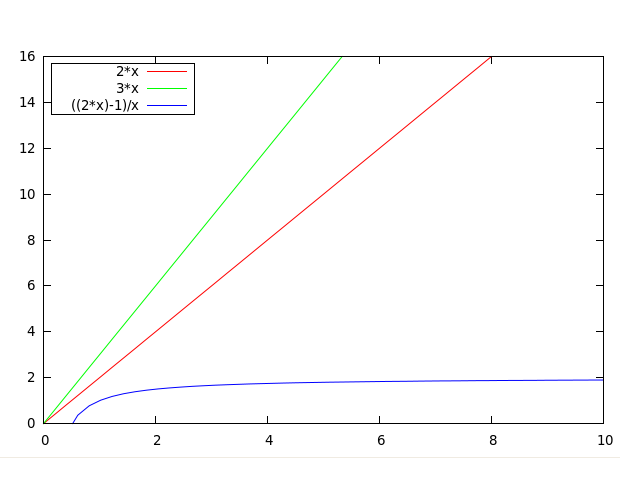
\includegraphics[scale=0.69]{figuras/gnuplot-replicacao-codificacao-3.png}
      \caption{Sobrecarga de armazenamento para replicação $3n$, $2n$ e codificação $(2k-1,k)$ representadas, respectivamente, pelas funções $y = 3x$, $y = 2x$ e $y = \frac{2x-1}{x}$, para $x>0$}
      \label{fig1:sarc}
    \end{figure}

Neste estudo, concluímos que a codificação por apagamento acarreta uma sobrecarga de armazenamento menor que a replicação para o mesmo número de falhas toleradas. 

Nas máquinas do Facebook, a codificação RS é (13, 10) com sobrecarga de ($B=1.3$) e tolera até 3 falhas por \emph{stripe}. A codificação XOR (RAID-5) é (11, 10) com sobrecarga de ($B=1.1$). Outro exemplo é a codificação RS(255, 223), utilizada pela DSN \cite{TDD:2010}, que é padrão CCSDS \footnote{http://public.ccsds.org/} e tolera 32 falhas com sobrecarga de $B=1.1435$. Uma codificação BCH(63, 56), também padrão CCSDS, pode tolerar até 7 falhas, dependendo do polinômio gerador da síndrome \cite{Almeida:2007} . 

\section{Disponibilidade dos nós}

\section{Leitura ou Atualização dos dados redundantes}

Em \cite{Chiola:2005}, os autores concluem que:

\begin{itemize}
  \item o acesso somente de leitura pode ser suportado tanto por replicação de dados simples como por codificação
  \item para privilegiar atualização consistente, uma codificação de alta disponibilidade é necessária que se caracteriza por fracionamento do original dados em pedaços $k$ e adicionando exatamente $k-1$ pedaços
  \item se ler e a disponibilidade de atualização consistente são de igual importância, isso requer codificação $(2k-1, k)$
\end{itemize}

Os autores também concluíram que usar apenas a replicação tem sentido apenas em poucos casos.

Concluímos que, apenas avaliando a contribuição do esquema de redundância, a codificação por apagamento 

Podemos também concluir que a replicação é um caso onde $k = 1$ e $l\ =\ m - k\ = \ n\ -\ 1$, portanto $m\ =\ n$. 
